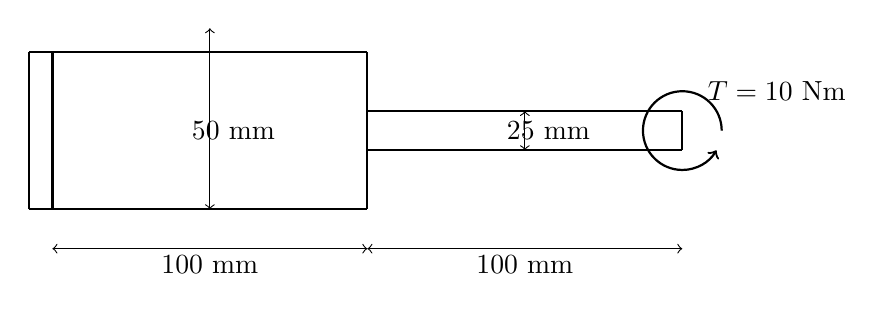
\begin{tikzpicture}
\usetikzlibrary{patterns}

% Left fixed support
\draw[thick] (0,0) -- (0,2); % Vertical line of support
\draw[thick] (0,0) -- (-0.3,0); % Bottom horizontal line of support
\draw[thick] (0,2) -- (-0.3,2); % Top horizontal line of support
\draw[thick, pattern=north east lines] (-0.3,0) -- (-0.3,2); % Hatching for fixed support

% Large shaft
\draw[thick] (0,0) -- (4,0); % Bottom edge of large shaft
\draw[thick] (0,2) -- (4,2); % Top edge of large shaft
\draw[thick] (4,0) -- (4,2); % Right edge of large shaft

% Small shaft
\draw[thick] (4,0.75) -- (8,0.75); % Bottom edge of small shaft
\draw[thick] (4,1.25) -- (8,1.25); % Top edge of small shaft
\draw[thick] (8,0.75) -- (8,1.25); % Right edge of small shaft

% Torque arrow
\draw[->,thick] (8.5,1) arc[start angle=0,end angle=330,radius=0.5]; % Circular arrow for torque

% Dimensions
\draw[<->] (0,-0.5) -- (4,-0.5); % Horizontal dimension line for large shaft
\draw[<->] (4,-0.5) -- (8,-0.5); % Horizontal dimension line for small shaft
\draw[<->] (2,2.3) --  (2,0); % Vertical dimension for large shaft height
\draw[<->] (6,0.75) --  (6,1.25); % Vertical dimension for small shaft height

% Labels
\node at (2,-0.7) {100 mm}; % Label for large shaft length
\node at (6,-0.7) {100 mm}; % Label for small shaft length
\node at (2.3,1) {50 mm}; % Corrected label placement for large shaft height
\node at (6.3,1) {25 mm}; % Corrected label placement for small shaft height
\node at (9.2,1.5) {$T = 10$ Nm}; % Corrected torque label position

\end{tikzpicture}

